\section{OpenCL}

\subsection{What is OpenCL?}
OpenCL is specified by the Khronos Group in the OpenCL 1.2 Specification as follows:

\begin{quotation}
OpenCL (Open Computing Language) is an open royalty-free standard for general purpose
parallel programming across CPUs, GPUs and other processors, giving software developers
portable and efficient access to the power of these heterogeneous processing platforms. \cite{opencl_spec}
\end{quotation}

The Khronos Group is an industry consortium who maintains OpenCL as an open standard. This means that the Khronos Group offers a specification of the OpenCL API and a detailed description about its functionality and behavior for free. This specification can be downloaded at their website \cite{opencl_spec}. Maintaining the OpenCL standard consequently means, that the Khronos Group neither provides software development kits (SDKs), drivers that implement OpenCL nor hardware that it can make use of. These concerns are subject to other companies called vendors, which are typically hardware manufacturers providing necessary developing resources and include OpenCL support in their drivers. Examples of such companies are the two famous graphic card vendors NVIDIA and AMD as well as the renowned processor manufacturer Intel.

Unlike other famous APIs the Khronos Groups specifies that are very specific in their usage or the targeted hardware (like the famous 3D API OpenGL used to drive graphic hardware), OpenCL is a general purpose programming framework. It was conceived with universality in mind offering almost no restrictions on the field of application it may be used. Portability from its well designed hardware abstraction model which enables it to run on many different kinds of devices, even ones which may have not been created yet, is one of OpenCL most powerful strengths. Such devices may be classical CPUs and GPUs, but also more uncommon types of hardware like FPGAs (field programmable gate arrays), DSPs (digital signal processors) or Intel's MICs (Many Integrated Core) \cite{mic}. Moreover, OpenCL may be used to combine multiple available devices into a single heterogeneous platform extending an applications processing resources beyond the bounds of individual pieces of hardware.

Additionally to being independent of a specific purpose and decoupled from the underlying hardware, OpenCL is also available across all mayor operations systems including Windows, Linux and Mac OS X.

With the upcoming specification of WebCL currently only available as a working draft, OpenCL will eventually even find its way into web browsers and the HTML5 technology conglomeration. Thus making it even independent of an operating system and bringing high performance computing into web applications.

\subsection{Components}

OpenCL is not an API alone. As it allows programs to run on hardware that may have certain restrictions or offer different features than a classical CPU, traditional languages like C++, Java or C\# can not be used to write those programs. Therefore, the OpenCL standard includes the specification of a separate language that is used to write small programs that are executed on a hardware device. These programs are called kernels and are written in the OpenCL C language, which is a restricted version of C99 with extensions for vectorization and handling OpenCL's abstract memory model.

The allow OpenCL to support many different hardware platforms it consists of the following components:

\begin{description}
	\item[API] \hfill \\
	The application programming interface is specified by the Khronos Group ensuring that every vendor implementation of OpenCL is compatible and exchangeable. The API is provided as a set of a C header files that a software developer can download from Khronos' website. These headers are typically also shipped within an SDK. Khronos additionally specifies a C++ wrapper for the C API. Bindings for other language exists but are not maintained by Khronos.
	The API is used by a conventional program (e.g. written in C++) to run kernels on an OpenCL capable device. This program is called the host application.
	\item[SDK] \hfill \\
	The software developing kit is the main collection of tools and resources a software developer needs to write applications using OpenCL. An SDK is usually provided by a vendor, an implementor of OpenCL. Examples of such SDKs are the NVIDIA CUDA Toolkit and AMD's Accelerated Parallel Processing (APP) SDK. These SDKs typically contain header files to be included by a C/C++ program and static libraries for the C/C++ linker which are responsible for binding to the OpenCL driver at runtime. Furthermore, code examples, tutorials, documentation, developing tools etc. may be additionally provided depending on the vendor. With headers and static libraries an SDK contains all resources necessary to write and compile an OpenCL application.
	\item[OpenCL C language] \hfill \\
	Kernels are typically written in separate source files using the OpenCL C language. An OpenCL application reads these source files at run time and sends them to the OpenCL compiler to create a binary for one or more available hardware devices where it may be executed. A source file written in the OpenCL C language may consist of several functions, variable definitions, control flow statements, comments, etc. but has to have at least one function prefixed with the \_\_kernel attribute, which may be called by the host application through the OpenCL API and serves as an entry point into a kernel.
	\item[OpenCL C Compiler] \hfill \\
	OpenCL kernels must be compiled for a specific platform before they can be executed. This compilation process is initiated and controlled by the host application through the API. This separate compilation at run time is required to retain OpenCL's portability as an OpenCL application may be deployed on any kind of machine with a suitable driver. As a result the available OpenCL implementation (providing the compiler) and the used hardware device (affecting the compiler's output) may only be determined at runtime.
	\item[Driver] \hfill \\
	Finally, the driver is OpenCL's core. It implements the OpenCL API and maps the functionality specified in the standard to a vendor's hardware. The host application uses the driver through the API to initialize OpenCL, compile kernels, allocate memory resources, initiate computations and communicate with kernels running on a device. A driver is always specific to a dedicated hardware and must therefore be provided by a vendor. The driver is sometimes also referred to as Installable Client Driver (ICD).
\end{description}

\subsection{Hardware architectures}

GPU /CPU hardware
similarities/differences

\subsection{Hardware abstraction}
platforms, devices, command queues, programs, kernels, buffers, ...

\begin{figure} % from http://http.developer.nvidia.com/CgTutorial/cg_tutorial_chapter01.html
\centering
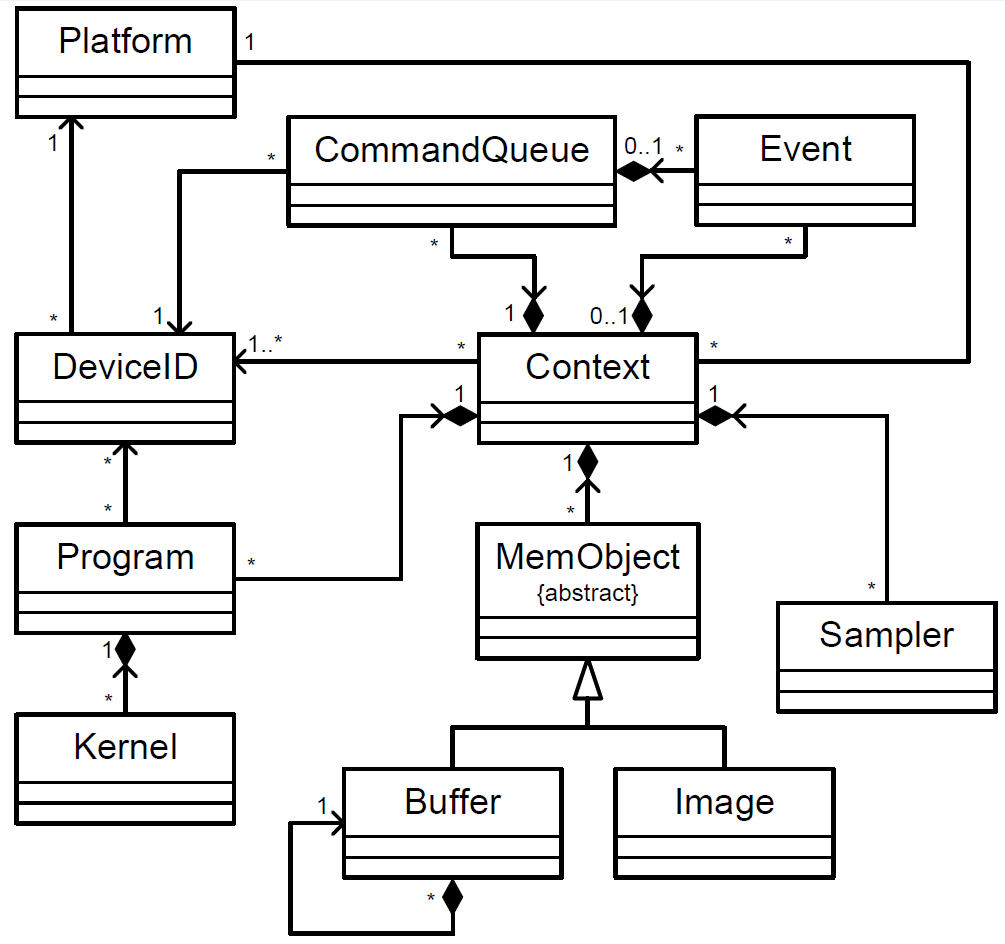
\includegraphics[width=0.7\linewidth]{opencl_uml}
\caption{OpenCL class diagram \cite{opencl_spec}}
\label{fig:opencl_uml}
\end{figure}

\subsection{Memory model}

\subsubsection{Types of memory}
different types of memory on the GPU
global local constant private
texture, pinned memory
performance
how do we access them?

\subsubsection{General design considerations}
coalesced memory access
local memory as programmable cache (and method of sync)
bench conflicts

\subsubsection{Data transfer}
read, write buffers
sync, async

\subsection{Kernel execution}
what is a kernel?

how are kernels executed?
work groups, work items
hardware threads (synchronization)

choosing the right work group size

\subsection{Structure of an OpenCL program}

with pseudocode example

